\documentclass[border=10pt]{standalone}
\usepackage{tikz}
\usetikzlibrary{arrows.meta, positioning, shapes.geometric}

\definecolor{blue1}{RGB}{0, 100, 180}
\definecolor{green1}{RGB}{50, 140, 50}
\definecolor{yellow1}{RGB}{190, 150, 0}
\definecolor{purple1}{RGB}{120, 80, 150}
\definecolor{gray1}{RGB}{120, 120, 120}

\begin{document}
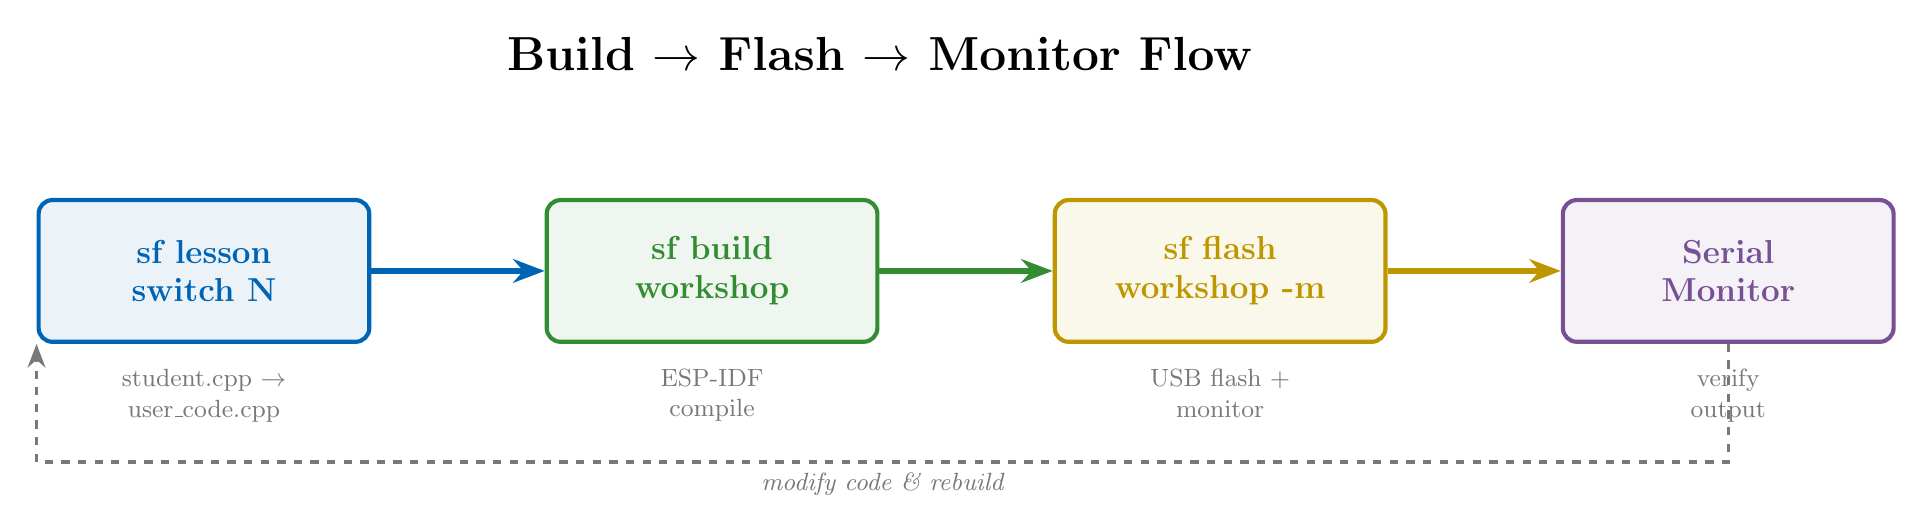
\begin{tikzpicture}[
    step/.style={
      rectangle, rounded corners=5pt, draw=#1, line width=1.5pt,
      fill=#1!8, minimum width=42mm, minimum height=18mm,
      font=\bfseries\large, text=#1, align=center
    },
    desc/.style={font=\small, text=gray1, align=center, below=2mm},
    arr/.style={-{Stealth[length=4mm]}, line width=2pt, #1},
    feedback/.style={-{Stealth[length=3mm]}, line width=1.2pt, gray1, dashed},
  ]

  % Steps
  \node[step=blue1] (s1) at (0, 0) {sf lesson\\switch N};
  \node[step=green1, right=22mm of s1] (s2) {sf build\\workshop};
  \node[step=yellow1, right=22mm of s2] (s3) {sf flash\\workshop -m};
  \node[step=purple1, right=22mm of s3] (s4) {Serial\\Monitor};

  % Arrows
  \draw[arr=blue1] (s1) -- (s2);
  \draw[arr=green1] (s2) -- (s3);
  \draw[arr=yellow1] (s3) -- (s4);

  % Descriptions
  \node[desc] at (s1.south) {student.cpp $\to$\\user\_code.cpp};
  \node[desc] at (s2.south) {ESP-IDF\\compile};
  \node[desc] at (s3.south) {USB flash +\\monitor};
  \node[desc] at (s4.south) {verify\\output};

  % Feedback loop
  \draw[feedback] (s4.south) -- ++(0, -1.5) -| node[pos=0.25, below, font=\small\itshape, text=gray1] {modify code \& rebuild} (s1.south west);

  % Title
  \node[font=\LARGE\bfseries, above=15mm of s2.north east] {Build $\to$ Flash $\to$ Monitor Flow};

\end{tikzpicture}
\end{document}
